Popis molekul v~rámci kvantové teorie je ústředním tématem kvantové chemie. Na rozdíl od atomů nejsou molekuly centrálně symetrické, což výpočty jejich vlastností komplikuje. V~důsledku nižší symetrie se tak například v~molekulách při elektronovém pohybu nezachovává moment hybnosti. V~případě molekul se musíme kromě pohybu elektronů vyrovnat také s~pohyby atomových jader. Atomová jádra jsou daleko těžší než elektrony, takže jejich popis na kvantové úrovni není vždy nezbytně nutný. Je ovšem třeba vědět, jaká jsou omezení klasického pohledu na atomová jádra. Díky rozdílné hmotnosti jader a elektronů můžeme pohyb atomových jader a elektronů (často) oddělit. To je podstatou tzv. Bornovy-Oppenheimerovy aproximace vedoucí ke konceptu hyperplochy potenciální energie. Tento koncept je pro chemika důležitý natolik, že si možná ani neuvědomí jeho přibližnou povahu.  


\subsection{Molekulový hamiltonián}


Nemělo by nám již být zatěžko zapsat pro molekulu hamiltonián. Ten musí obsáhnout všechny molekulové interakce mezi jádry a elektrony. Při zanedbání relativistických efektů nabývá následujícího tvaru

\begin{equation}
\hat{H}=\hat{T}_R+\hat{T}_r+\hat{V}_{nn}+\hat{V}_{nr}+\hat{V}_{rr}, 
\label{rov:mol-Hamiltonian}
\end{equation}

\noindent kde $\hat{T}_R$ je operátor kinetická energie jader

\begin{equation}
\hat{T}_R=\sum_i	-\frac{\hbar^2}{2m_{n,i}}\Delta_{i}, 	
\end{equation}

\noindent $\hat{T}_r$ operátor kinetická energie elektronů

\begin{equation}
\hat{T}_r=\sum_j	-\frac{\hbar^2}{2m_{e}}\Delta_{j}, 	
\end{equation}

\noindent $\hat{V}_{nn}$ popisuje coulombovské odpuzování mezi jádry

\begin{equation}
\hat{V}_{nn}=\frac{1}{4\pi\epsilon_0}\sum_i\sum_{i'>i}\frac{Z_iZ_{i'} e^2}{ \left\vert \textbf{R}_i - \textbf{R}_{i'}\right\vert } , 	
\end{equation}

\noindent $\hat{V}_{nr}$ popisuje přitahování mezi jádry a elektrony
\begin{equation}
\hat{V}_{nr}=\frac{1}{4\pi\epsilon_0}\sum_i\sum_j\frac{Z_i e^2}{ \left\vert \textbf{R}_i - \textbf{r}_j\right\vert } , 	
\end{equation}

\noindent a $\hat{V}_{rr}$ popisuje odpuzování mezi elektrony

\begin{equation}
\hat{V}_{rr}=\frac{1}{4\pi\epsilon_0}\sum_j\sum_{j'>j}\frac{ e^2}{ \left\vert \textbf{r}_j - \textbf{r}_{r'}\right\vert }. 	
\end{equation}

\noindent Ve výše uvedených výrazech jsou $\textbf{R}_i$ a $\textbf{r}_j$ symboly pro polohové vektory pro jádro $i$ a elektron $j$, $Z_i$ pak značí nábojové číslo jádra $i$. Naším úkolem je vyřešit Schrödingerovu rovnici

\begin{equation}
\hat{H}\psi=E\psi
\end{equation}

\noindent kde vlnová funkce $\psi$ je funkcí jak souřadnic elektronů, tak souřadnic atomových jader. 

\subsection{Bornova-Oppenheimerova aproximace}

Přesné řešení Schrödingerovy rovnice s~molekulovým hamiltoniánem je mimořádně komplikované. Situaci nám ale hodně zjednoduší oddělení pohybu elektronů a atomových jader v~rámci \textbf{Bornovy-Oppenheimerovy aproximace} (BOA). Nejprve se na BOA podíváme stručně s~nadhledem, poté již budeme matematicky rigoróznější. 

\subsubsection{Bornova-Oppenheimerova aproximace: První pohled}


I~nejlehčí atomové jádro (proton) je přibližně 1800krát těžší než elektron.  Pohybuje se proto také mnohem pomaleji než elektron. Kvantový elektron tak v~každé chvíli vidí v~podstatě stojící, klasická atomová jádra. Pro každou geometrii jader můžeme proto vyřešit elektronovou Schrödingerovu rovnici a vypočítat příslušnou energii, se kterou se elektrony v~molekule v~dané geometrii pohybují

\begin{equation}
\hat{H}_{el}\psi_{el}=E_{el}\psi_{el},
\end{equation}

\noindent kde $\hat{H}_{el}$ je elektronový hamiltonián

\begin{equation}
\hat{H}_{el}=\hat{T}_r+\hat{V}_{nr}+\hat{V}_{rr}+\hat{V}_{nn}
\end{equation}

\noindent a $E_{el}$ je elektronová energie (energie, se kterou se v~molekule pohybují elektrony, tato energie v~sobě většinou zahrnuje i coulombovské odpuzování mezi atomovými jádry). $\psi_{el}$ je pak elektronová vlnová funkce. Ta je funkcí souřadnic elektronů $\textbf{r}_j$, parametricky je ale závislá i na souřadnicích atomových jader. Pojmem \uv{parametrická závislost} máme na mysli, že elektronová vlnová funkce bude jiná pro každou geometrii $\textbf{R}_i$ a pro každou geometrii spočítáme také jinou elektronovou energii $E_{el}$. 

Závislost elektronové energie na souřadnicích atomových jader se pro dvouatomové molekuly nazývá křivkou potenciální energie, pro víceatomové molekuly potom hyperplochou potenciální energie. Hyperplocha potenciální energie je ústřední pojem teoretické chemie, který dává chemikovi jasnou představu o~struktuře a reaktivitě molekul. 

\begin{figure} [ht]
\centering
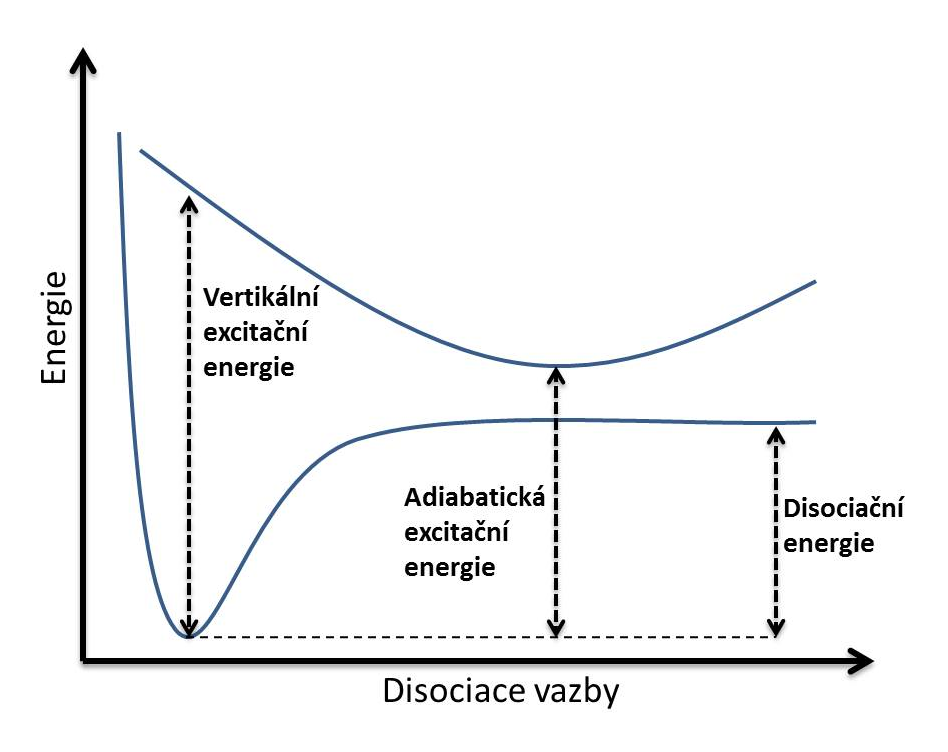
\includegraphics[scale=0.6]{obrazky/disociace2.eps}
\caption[Disociace]{Co lze vyčíst z~hyperplochy potenciální energie.}
\label{obr:mol:disociace2}
\end{figure}

Obrázek~\ref{obr:mol:disociace2} znázorňuje křivku potenciální energie pro obecný případ dvouatomové molekuly. Křivky jsou vykresleny pro dva elektronové stavy. Na těchto křivkách jsou vyznačeny rovnovážné geometrie v~základním a v~excitovaném stavu a některé významné energetické údaje.


Hyperplochu potenciální energie si nyní ukážeme na několika konkrétních příkladech. Obrázek~\ref{obr:mol:H2_Ar} zobrazuje hyperplochy potenciálních energií pro $\mathrm{H}_2^+$ a dvouatomový komplex argonu. Hyperplocha (nebo v~tomto případě křivka) potenciální energie nám říká, jak na sebe působí atomy či molekuly. Podívejme se nejprve křivku potenciální energie $\mathrm{H}_2^+$. Modrá křivka zobrazující základní elektronový stav má minimum ve vzdálenosti kolem 0,1~nm. Tato vzdálenost odpovídá rovnovážné geometrii molekuly $\mathrm{H}_2^+$ . Červená křivka znázorňující elektronově excitovaný stav naopak žádné minimum nemá. Energie tohoto stavu je tím nižší, čím jsou atomy vodíku dál od sebe. Z~této křivky vidíme, že molekula $\mathrm{H}_2^+$ se v~excitovaném stavu rozpadne.

\begin{figure} [ht]
\centering
\begin{center}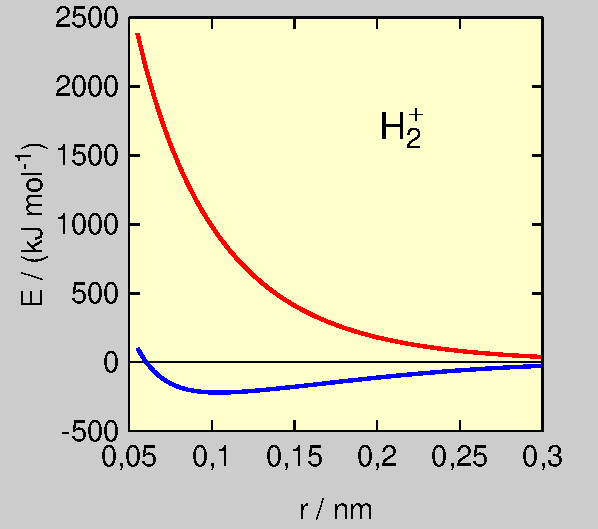
\includegraphics[scale=0.8]{obrazky/h2+.pdf}\hspace*{-1pt}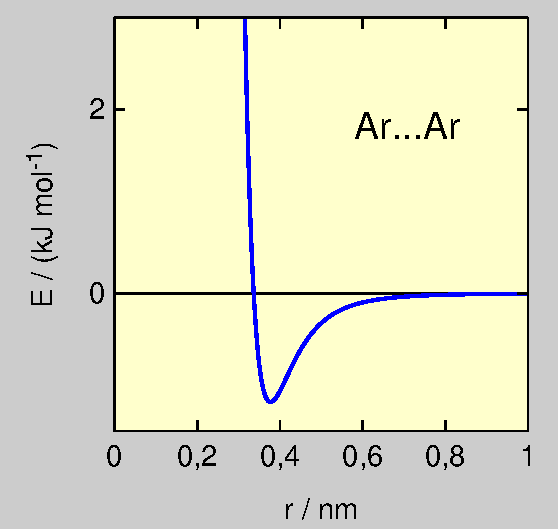
\includegraphics[scale=0.8]{obrazky/arar.pdf}\end{center}
\caption[Křivky potenciální energie]{Křivky potenciální energie pro $\mathrm{H}_2^+$ a dvouatomový komplex argonu. Energie v~obou případech byly vypočítány řešením stacionární Schrödingerovy rovnice.}
\label{obr:mol:H2_Ar}
\end{figure}

Druhý obrázek znázorňuje dva atomy argonu. Ze střední školy si všichni pamatujeme, že vzácné plyny netvoří dvouatomové molekuly. Křivka potenciální energie argonu nicméně vykazuje minimum. Nejde však o~chemickou vazbu. Všimněme si, že energetické minimum pro argon je mnohem dál než minimum pro $\mathrm{H}_2^+$. Navíc, podíváme-li se na energetickou osu, všimneme si, že minimum u~argonu není ani zdaleka tak hluboké jako bylo v~případě $\mathrm{H}_2^+$. Argon vskutku netvoří chemické vazby, ale je stabilizován pouze slabými nekovalentními interakcemi, konkrétně tzv. disperzními silami.


\begin{figure} [ht]
\centering
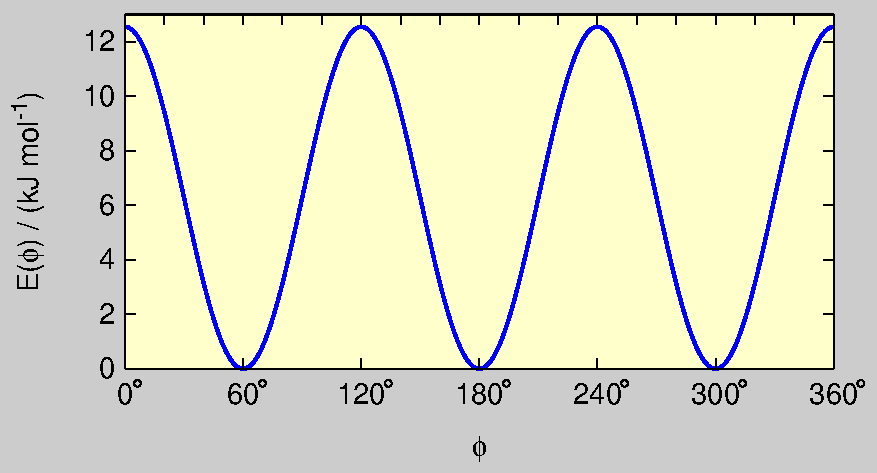
\includegraphics[scale=0.9]{obrazky/ethane.pdf}
\caption[Torzní bariéra ethanu]{Závislost potenciální energie na vzájemném otáčení methylových skupin v~molekule ethanu.}
\label{obr:mol:ethan}
\end{figure}

Další příklad si vypůjčíme ze základního kurzu organické chemie. Molekula ethanu obsahuje dvě methylové skupiny. Pokud jednu methylovou skupinu otočíme, bude se měnit potenciální energie (tj. elektronová energie) této molekuly. Dva limitní příklady nazýváme zákrytová a~nezákrytová konformace. Obrázek~\ref{obr:mol:ethan} ukazuje energetiku otáčení methylové skupiny, přičemž všechny energie byly opět vypočítány řešením stacionární Schrödingerovy rovnice.

\begin{figure} [ht]
\centering
\begin{center}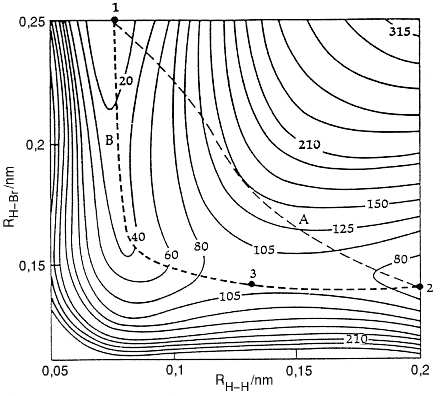
\includegraphics[scale=1.0]{obrazky/potsurface1.pdf}\hfill\raise 2mm\hbox{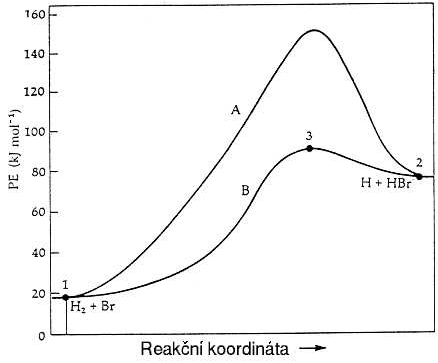
\includegraphics[scale=1.0]{obrazky/potsurface2.pdf}}
\end{center}
\caption[Potenciální energie reakce Br + HBr]{Vrstevnicový diagram potenciální energie pro reakci Br + HBr.}
\label{obr:mol:HBr}
\end{figure}

Poslední příklad nám ukáže, že pojem hyperplocha potenciální energie je důležitý také v~chemické kinetice. Podívejme se na vznik bromovodíku podle následující reakce

\begin{equation}
\mathrm{H}_2+\mathrm{Br}\longrightarrow\mathrm{HBr}+\mathrm{H}, 
\end{equation} 

\noindent kde se přenese atom vodíku k~bromu, jedna chemická vazba zanikne a druhá vznikne. Elektronová energie systému o~třech atomech závisí na třech souřadnicích, což již ve dvou rozměrech neznázorníme. Vybereme si proto jenom dvě souřadnice, vzdálenost mezi dvěma atomy vodíku a vzdálenost mezi atomem vodíku a atomem bromu. Závislost energie na geometrii pak znázorníme pomocí vrstevnicového diagramu (viz obrázek~\ref{obr:mol:HBr}). Údaje ve vrstevnicovém diagramu odečítáme podobně jako v~mapě. Analogicky také hledáme nejméně náročnou cestu od reaktantů k~produktů, tj. údolím reaktantů přes sedlo k~údolí produktů (obrázek znázorňuje ještě jinou, energeticky náročnější konkurenční reakční cestu). Takovéto reakční cestě říkáme reakční koordináta. V~pravé části obrázku pak vidíme energetický profil reakce podél této reakční koordináty. 

Hyperplocha potenciální energie je smysluplný pojem pouze pokud je pohyb atomových jader a elektronů je nezávislý. Matematicky tuto nezávislost formulujeme tak, že celkovou vlnovou funkci zapíšeme jako součin vlnové funkce elektronů ($\psi_{el}$) a vlnové funkce jader ($\chi$)

\begin{equation}
\boxed{\psi=\chi(\textbf{R})\psi_{el}(\textbf{r};\textbf{R}).}
\label{rov:mol-BO}
\end{equation}


\subsubsection{Bornova-Oppenheimerova aproximace: Odvození}
Vyjdeme z~elektronového hamiltoniánu, který popisuje elektrony pro stojící jádra v~konkrétní geometrii $\textbf{R}_i$

\begin{displaymath}
\hat{H}_{el}=\hat{T}_r+\hat{V}_{nr}+\hat{V}_{rr}+\hat{V}_{nn}.
\end{displaymath}

\noindent Elektronový hamiltonián působí toliko na funkce souřadnic elektronů (přičemž ale tento elektronový hamiltonián je různý pro různé souřadnice jader $\textbf{R}_i$). Vyřešme nejdříve pro každou z~možných geometrií elektronovou Schrödingerovu rovnici

\begin{equation}
\boxed{\hat{H}_{el}\psi_{el}^{(i)}=E_{el}^{(i)}\psi_{el}^{(i)}.}
\end{equation}

\noindent Znovu připomeňme, že řešením je vlnová funkce souřadnic elektronů parametricky závislá na souřadnicích jader

\begin{equation}
\psi_{el}^{(i)}=\psi_{el}^{(i)}(\textbf{r}; \textbf{R}).
\end{equation}

\noindent Pod pojmem \uv{parametrická závislost} máme na mysli, že vlnová funkce je různá pro různé souřadnice jader, přičemž ale čtverec vlnové funkce nemá význam hustoty pravděpodobnosti nalezení jader v~určité geometrii $\textbf{R}_i$. Sada vlastních funkcí elektronového hamiltoniánu vytváří úplný soubor funkcí a můžeme tedy každou funkci souřadnic elektronů rozvinout do báze vlastních funkcí elektronového hamiltoniánu. Můžeme to učinit i pro celkovou vlnovou funkci

\begin{equation}
\psi(\textbf{r},\textbf{R})=\sum_i \chi_i(\textbf{R})\psi_{el}^{(i)}(\textbf{r}; \textbf{R}),
\label{rov:mol-BO2}
\end{equation}

\noindent kde $\chi_i(\textbf{R})$ jsou rozvojové koeficienty, které závisí na poloze jader. Doposud jsme se nedopustili žádné aproximace. Dosadíme tedy vlnovou funkci $\psi(\textbf{r},\textbf{R})$ do Schrödingerovy rovnice $\hat{H}\psi=E\psi$, jejíž levou stranu si dále upravíme

\begin{equation}
\hat{H}\psi=\sum_i (\hat{T}_R+\hat{H}_{el})\chi_i\psi_{el}^{(i)}=\sum_i \left[\hat{T}_R(\chi_i\psi_{el}^{(i)}) + \chi_iE_{el}^{(i)}\psi_{el}^{(i)}\right].
\label{rov:mol-mat2}
\end{equation}

\noindent Nyní si upravíme první člen pravé strany poslední rovnice. Výklad zjednodušíme tím, že budeme uvažovat operátor kinetické energie pouze v~jednom rozměru, tj. 

\begin{displaymath}
\hat{T}_R=\frac{-\hbar^2}{2m_R}\frac{\mathrm{d}^2}{\mathrm{d}R^2}.
\end{displaymath}

\noindent Nyní se zaměříme na působení operátoru kinetické energie jader

\begin{equation}
\hat{T}_R\chi_i\psi_{el}^{(i)}=\frac{\hbar^2}{2m_R}\left(
\psi_{el}^{(i)}\frac{\mathrm{d}^2\chi_i}{\mathrm{d}R^2}
+2\frac{\mathrm{d}\chi_i}{\mathrm{d}R}\frac{\mathrm{d}\psi_{el}^{(i)}}{\mathrm{d}R}+\chi_i\frac{\mathrm{d}^2\psi_{el}^{(i)}}{\mathrm{d}R^2}
\right)
\label{rov:mol-BOmat}
\end{equation}

\noindent Na tomto místě se dopustíme aproximace: zanedbáme poslední dva členy z~rovnice \ref{rov:mol-BOmat}, tedy
 
\begin{equation}
\hat{T}_R\chi_i\psi_{el}^{(i)}\approx\frac{\hbar^2}{2m_R}
\psi_{el}^{(i)}\frac{\mathrm{d}^2\chi_i}{\mathrm{d}R^2}.
\end{equation}

\noindent Z~odvození Bornovy-Oppenheimerovy aproximace jasně vidíme, že obecně bude platit tím lépe, čím méně se bude elektronová vlnová funkce měnit s~geometrií. Můžeme hned nabýt podezření, že pro rychle se pohybující jádra by Bornova-Oppenheimerova aproximace nemusela fungovat úplně dobře.

Vraťme se ještě k~rovnici \ref{rov:mol-mat2}. Rovnici nejprve vynásobíme komplexně sdruženou elektronovou vlnovou funkcí $\psi_{el}^{j}$ a následně prointegrujeme přes souřadnice elektronů $r$

\begin{equation}
\sum_i \left[\hat{T}_R(\chi_i\psi_{el}^{(i)}) + \chi_iE_{el}^{(i)}\psi_{el}^{(i)}\right]=E\sum_i \psi_{el}^{(i)}\chi_i \qquad \qquad /.\psi_{el}^{(j)*},/\int d\tau
\end{equation}


\noindent Schrödingerova rovnice (v~jedné dimenzi) nabude tvaru
\begin{equation}
\sum_i \left[\hat{T}_R\chi_i\int\psi_{el}^{(j)*}\psi_{el}^{(i)}d\tau + \chi_iE_{el}^{(i)}\int\psi_{el}^{(j)*}\psi_{el}^{(i)}d\tau\right]=E\sum_i \int \psi_{el}^{(j)*}\psi_{el}^{(i)}\chi_id\tau. 
\end{equation}
Vzhledem k~tomu, že elektronové vlnové funkce jsou ortonormální, rovnice se zjednoduší na následující tvar
\begin{equation}
\sum_i \left[\hat{T}_R\chi_i\delta_{ij} + \chi_iE_{el}^{(i)}\delta_{ij}\right]=E\sum_i \int \delta_{ij}\chi_i. 
\end{equation}
Kroneckerovo $\delta$ nám nakonec vybere pouze členy pro $i=j$

\begin{equation}
\boxed{\left(\hat{T}_R+E_{el}^{(j)}\right)\chi_j=E\chi_j.}
\label{rov:mol-jadschr}
\end{equation}

\noindent Rovnice \ref{rov:mol-jadschr} představuje Schrödingerovu rovnici pro jádra. Vidíme, že jádra se pohybují v~potenciálu daného elektronovou energií pro jednotlivé geometrie. 

\subsubsection{Meze platnosti Bornovy-Oppenheimerovy aproximace}

Není těžké naleznout příklady, kdy Bornova-Oppenheimerova aproximace selhává. Vezměme si molekulu chloridu sodného (viz obrázek~\ref{obr:mol:NaCl disociace}). NaCl je v~základním stavu vázána iontovou vazbu, minimum základního stavu si tedy můžeme přibližně popsat jako $\mathrm{Na}^{+}\mathrm{Cl}^{-}$. Když od sebe oddalujeme atomy chloru a sodíku, roste energie, až dojde k~rozpadu chemické vazby. Molekula se může rozpadnout dvěma způsoby, na $\mathrm{Na}^{+}$ a $\mathrm{Cl}^{-}$ nebo na $\mathrm{Na}$ a $\mathrm{Cl}$, přičemž jedna limita odpovídá základnímu a druhá excitovanému stavu. Nyní uvažujme, že molekulu chloridu sodného excitujeme. Kovalentně vázaný excitovaný stav v~geometrii globálního minima není stabilní a bude se proto rozpadat. Tento rozpad by se dle Bornovy-Oppenheimerovy aproximace měl odehrávat na jedné křivce potenciální energie a výsledkem by tak měly být ionty $\mathrm{Na}^{+}\mathrm{Cl}^{-}$. Ve skutečnosti vzniknou oba produkty, jak iontový, tak kovalentní. V~oblasti křížení stavů se totiž elektronová vlnová funkce s~mezijadernou vzdáleností dramaticky mění a druhý a třetí člen v~rovnici \ref{rov:mol-BOmat} proto není možno zanedbat. 


\begin{figure} [ht]
\centering
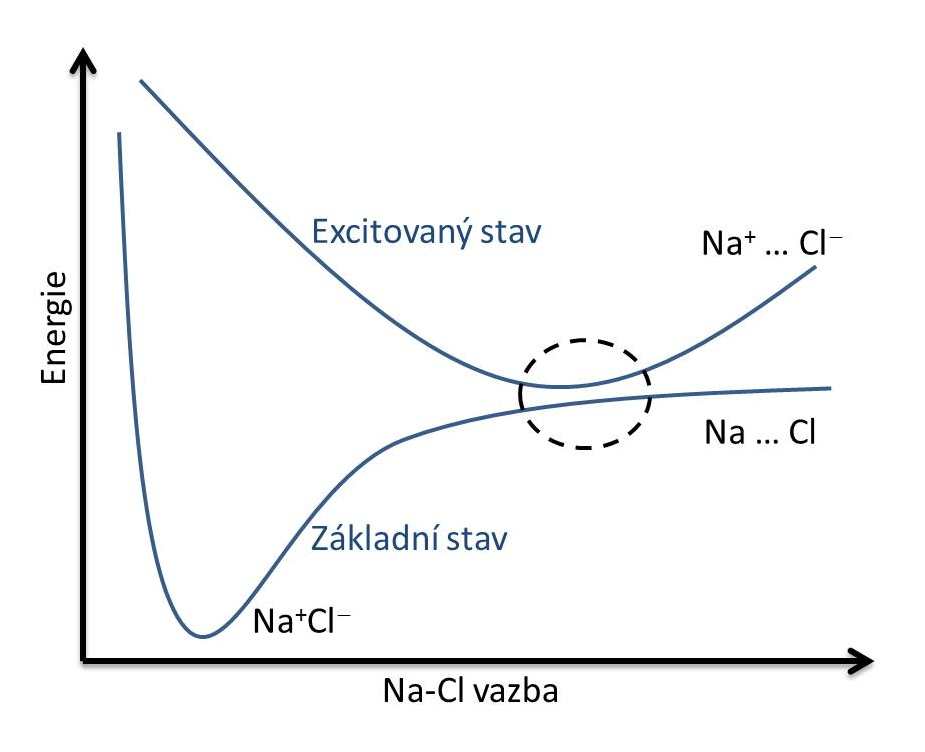
\includegraphics[scale=0.5]{obrazky/NaCl_disociace.eps}
\caption[NaCl disociace]{Ukázka selhání Bornovy-Oppenheimerovy aproximace}
\label{obr:mol:NaCl disociace}
\end{figure}


 
